\documentclass{article}
\usepackage{graphicx} % Required for inserting images
\usepackage[utf8]{inputenc}
\usepackage{amsmath, wrapfig}
\usepackage[letterpaper, margin = 1in]{geometry}
\usepackage{asymptote, amssymb}
\usepackage{setspace}
\setlength{\parindent}{0cm}
\usepackage[inline]{asymptote}
\usepackage[english]{babel}
\usepackage{amsthm, amssymb, amsmath, fancyhdr, mathtools}
\usepackage{asymptote}
\usepackage{hyperref}
\setcounter{section}{-1}
\usepackage[letterpaper, left=1.5cm, right=1.5cm, top=2cm, bottom=2cm,]{geometry}
\usepackage{etoolbox}
\usepackage{enumitem}
\usepackage{framed}
\renewenvironment{leftbar}[1][\hsize]
{%
    \def\FrameCommand
    {%
        %{\color{red}\vrule width 3pt}%
        %\fboxsep=\FrameSep\colorbox{yellow}%
        {\vrule width 3pt}%
        \hspace{10pt}%must no space
    }%
    \MakeFramed{\hsize#1\advance\hsize-\width\FrameRestore}%
}
{\endMakeFramed}
\newenvironment{quotationb}%
{\begin{leftbar}\begin{quotation}}%
{\end{quotation}\end{leftbar}}

\pagestyle{fancy}
\newtheoremstyle{problem}% <name>
{3pt}% <Space above>
{3pt}% <Space below>
{}% <Body font>
{}% <Indent amount>
{\bfseries}% <Theorem head font>
{.}% <Punctuation after theorem head>
{.2em}% <Space after theorem headi>
{}% <Theorem head spec (can be left empty, meaning `normal')>
\newtheorem{theorem}{Theorem}
\AfterEndEnvironment{theorem}{\noindent}
\newtheorem*{corollary}{Corollary}
\newtheorem*{lemma}{Lemma}

\newtheorem{proposition}{Proposition}
\theoremstyle{remark}

\newtheorem*{solution}{Solution}
\AfterEndEnvironment{solution}{\noindent}

\newtheorem*{example}{Example}
\theoremstyle{problem}

\newtheorem{problem}{Problem}
\AfterEndEnvironment{problem}{\noindent}

\numberwithin{problem}{subsection}
\newtheorem{Problem}{Problem}

\AfterEndEnvironment{Problem}{\noindent}
\numberwithin{Problem}{section}

\theoremstyle{definition}
\newtheorem*{definition}{Definition}
\theoremstyle{definition}


\newtheorem{conjecture}{Conjecture}
\theoremstyle{definition}

\newtheorem*{remark}{Remark}
\newcommand{\andd}{\wedge}
\newcommand{\orr}{\vee}
\usepackage{kpfonts}
\DeclareMathOperator{\var}{var}
\setlength\parindent{24pt}
\newcommand{\probP}{\text{I\kern-0.15em P}}

\title{The Collatz Conjecture}
\author{Nishka Kacheria}
\date{November 2023}

\doublespacing 

\begin{document}
\lhead{Nishka Kacheria}

\maketitle

\section{Introduction}
The Collatz conjecture has the infamy of a black hole. Young, promising mathematicians are sucked into it, never to be seen again, because this conjecture has been unsolved for so long (and is quite difficult, as expected). 

The statement of the Collatz conjecture is that $\forall n \in \mathbb{N^{+}} $ and a function $f(n)$ operating on it repeatedly, where 
$$f(n) = \begin{cases}
    3n + 1 \text{ if n is odd} \\
    \frac{n}{2} \text{ if n is even}
\end{cases}$$
the sequence of $n, f(n), f(f(n)), f(f(f(n))) \cdots $ will eventually reach $1.$

Additionally, the aforementioned sequence is referred to as the Collatz sequence. 

As can be seen, it is simple to state, and yet there are still no solutions. 
A good introductory video to the conjecture can be found here: https://www.youtube.com/watch?v=094y1Z2wpJg by Veritasium. 

Intuitively, the Collatz Conjecture makes sense. The of growth for $n$ in the function is $\frac{3}{4} < 1,$ implying that the conjecture does eventually converge at $1$ (Veritasium). 

One might think that the growth rate is $\frac{3}{2},$ implying that sequences will eventually diverge, since $n$ either increases by a factor of $3$ or decreases by a factor of $\frac{1}{2}.$ Since both cases happen with roughly equal probability (half of all numbers are odd, the other half are even), we can say that the overall growth factor is likely to be about $3 \cdot \frac{1}{2} = \frac{3}{2}$

However, for all odd numbers, $3n + 1$ yields an even number (as 3 times an odd number is still odd, adding 1 makes it even). This means that we know the next move will be to divide the new value by 2, and then the parity of the number is random. This means that we can instead consider 

$$f(n) = \begin{cases}
    \frac{3n + 1}{2} \text{ if n is odd} \\
    \frac{n}{2} \text{ if n is even}
\end{cases}$$

And thus the growth rate is, on average, $\frac{3}{2} \cdot \frac{1}{2} = \frac{3}{4},$ which does imply an eventual convergence. 

\section{Interesting Facts}

There are several interesting observations on the Collatz conjecture that are also pretty basic and serve as a nice introduction.

\begin{enumerate}
    \item The Collatz conjecture can never yield a number that is a multiple of 3 except at the very beginning of the sequence, since all odd terms become $1 \bmod 3$ and all even terms cannot gain a factor of $3.$ This means, for example, that when looking at the numbers in Collatz sequences, only $\frac{2}{3}$ of the natural numbers could be used in the sequence.
\end{enumerate}

\section{Cycle}

The Collatz conjecture includes the following:

\begin{conjecture}
    The only positive integer cycle (where the repeated application of $f(n)$ reaches a value previously reached) is $4, 2, 1.$ As is evident, $4/2 = 2, 2/2 = 1,$ and $3(1) + 1 = 4.$
\end{conjecture}

An important theorem that initially guided cycle length calculation follows.
\begin{theorem}
 Define $k$ as the number of $3x + 1$ operations, and $n$ as the number of $\frac{x}{2}$ operations. If there is a cycle besides the 4-2-1 cycle, name it's lowest element as greater than some number $R.$ Then,

$$ \log_{2}(3) < \frac{n}{k} \leq \log_{2} \left( 3 + \frac{1}{R} \right)$$

(Sinisalo 2003).
\end{theorem}

We can continue with the proof!

\begin{proof}
    Denote the Collatz sequence of values in the cycle such that each consecutive term is the result of applying the recursive function on the previous value. Denote this sequence $ c_1, c_2, \hdots , c_m.$ Additionally, note that $c_1$ is the result of the Collatz function applied to $c_m.$

    Now, let's look at the ratios of the successive terms in the sequence. This would be $$\frac{c_2}{c_1} \cdot \frac{c_3}{c_1} \cdots \frac{c_1}{c_m}.$$ Trivially, this telescoping series is equal to 1.

    Then, note that every one of the $n$ operations where the previous value is divided by two has a ratio of $\frac{1}{2}.$ This means that these values, multiplied, give $\frac{1}{2^n}.$ For the series above to equal 1, the product of the ratios of successive elements in each of the $k$ elements must also equal $2^{n}.$

    Then, note that the ratio of successive elements for each of the $k$ elements is also greater than $3$ and less than $\frac{3 c_1 + 1}{c_1}$ (since we are operating $3x + 1$) and $c_1$ is the first and smallest value without loss of generality. 

    This means that the product of each of these ratios is bounded by $3^k$ and $\left( 3 + \frac{1}{c_1} \right)^k.$

    Thus, we can construct the following inequality: $$3^k < 2^n \leq \left( 3 + \frac{1}{c_1} \right)^k. $$

    Taking $log_{2}$ of each section of the expression, and applying the log rule $ \log (b^k) = k \log (b),$ we get that $$ k \log_{2}{3} < n \leq k \log_{2} \left( 3 + \frac{1}{R} \right),$$ and dividing all parts by $k,$ we get that $$ \log_{2}(3) < \frac{n}{k} \leq \log_{2} \left( 3 + \frac{1}{R} \right).$$

\end{proof}

This can be used for the following theorem:

\begin{theorem}
     Let $\frac{a}{b}$ be the rational number with least possible denominator $b$ such that $ \log_{2}(3) < \frac{a}{b} \leq \log_{2} \left( 3 + \frac{1}{R} \right).$ Then, the least possible cycle length for a new cycle (not 4-2-1) is $a + b$ (Sinisalo 2003).
\end{theorem}
    
\begin{proof}
    A rigorous proof requires math outside the scope of this article, but can be found here! https://www.probleme-syracuse.fr/cargo/Sinisalo\_collatz.pdf. 

    However, a rough outline of the proof comes from taknig the floor function on this theorem and coming up with integer bounds for the values of $a$ and $b,$ as well as noting that $a + b = n + k,$ and using this to prove the theorem!
\end{proof}

Then, calculating the actual value of $\frac{a}{b}$ gives $630,138,897/397,573,379.$ The total length of a cycle is thus greater than $1,027,712,276.$

Thus, we have a huge lower bound, which is helpful! We are likely to be able to push this bound up even higher. In fact, Tomas Oliveira e Silva confirmed with a computer that all Collatz sequences with initial values up to $3 \cdot 2^{53} \approx 2.702 \times 10^{16}$ converge to the 4-2-1 cycle.

Another significant advancement in looking at cycles came in 2019 when Terrence Tao proved essentially the name of his paper "Almost all Collatz orbits attain almost bounded values." He  proved the Collatz Conjecture for almost all numbers, and with the following theorem: 

\begin{theorem}
    For any function $g(n)$ of positive integers such that $lim_{n \to \infty} g(n) \to \infty,$ the minimal value of the Collatz sequence must be less than or equal to $g(n)$ for the starting integer $n$ in the Collatz sequence (Tao 2019).
\end{theorem}

A simple example of this is just ascending integers: $1, 2, \cdots$. This theorem thus proves that the minimal value in a Collatz sequence starting with $n$ is always less than $n.$ 



\section{Stopping Times}

\begin{definition}
    The stopping time of a number as the amount of iterations before a number reaches $1.$ 
\end{definition}

A lot of work has been done for the Collatz conjecture, but there has not been as much analysis on the actual stopping times - namely, which values are most common for the stopping time of a function and how the stopping times are viewed. 

Graphing the stopping times with transitions is rather unhelpful due to the density of the lines. 

\begin{centering}
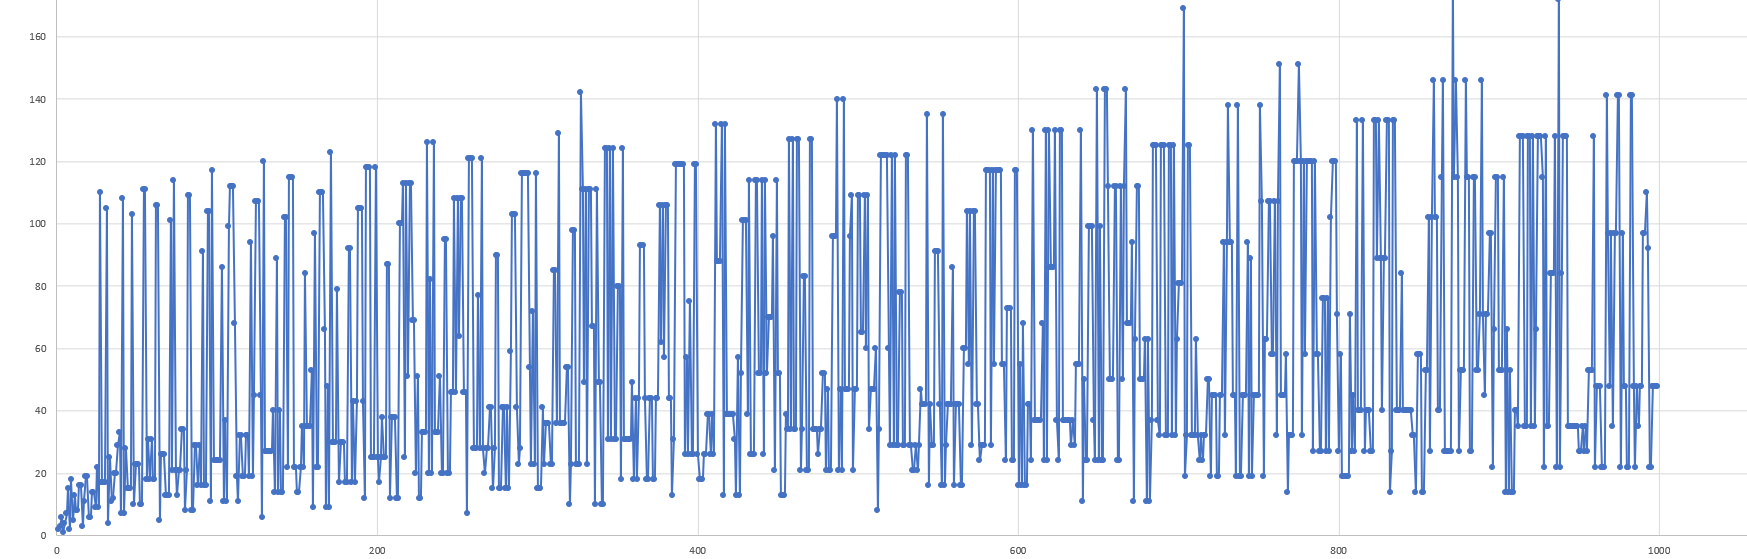
\includegraphics[width = \textwidth]{Pictures/1000 Collatz Stopping Times with Lines.png}
\end{centering}

Removing the connections between adjacent points, we can see the following graph of stopping times.

I calculated these stopping times just by running the recursive function, and with dynamic programming to speed up the process. Still, it was extremely fast, and easily replicable.


\begin{wrapfigure}{L}{0.7 \textwidth}
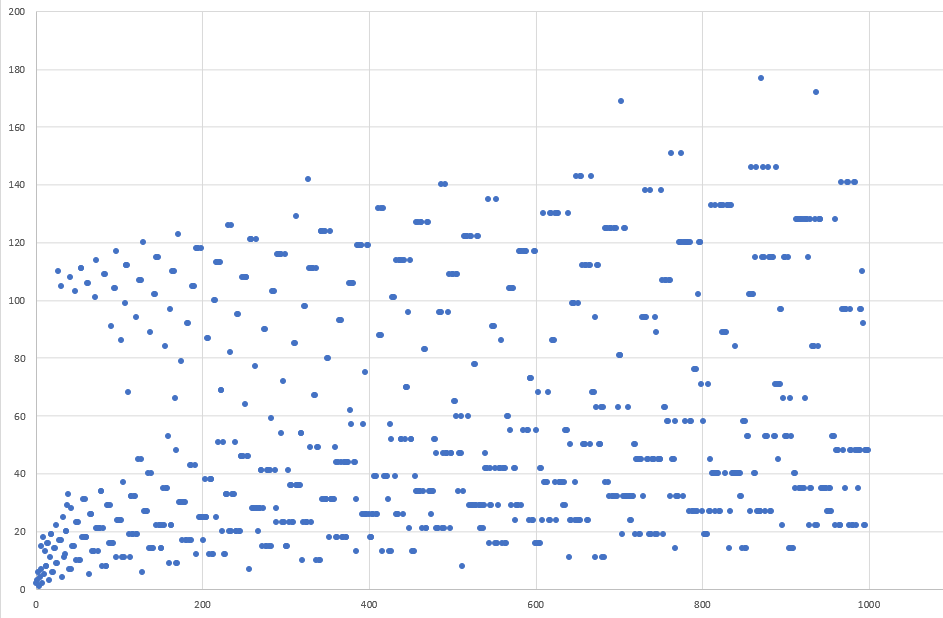
\includegraphics[width = 0.7 \textwidth]{images/1000 Collatz Stopping Times.png}

\end{wrapfigure}

In fact, we can predict that this pattern will probably continue to a higher number of x-values, too. It is a pretty pattern, and there seems to be a few different values that have the highest amount of stopping times - clustered around 105, and around 25. A paper by Lagarias from 1985 presents similar results for the range just beyond 1000, with a continued cluster at 23 and at 80, both different numbers in terms of primality and value. It's strange!


\begin{centering}
    \includegraphics[width=\textwidth]{images/Collatz Stopping Times Lagarias.png}
\end{centering}

To confirm the continued pattern, we can look at 10,000 datapoints. 

\begin{centering}
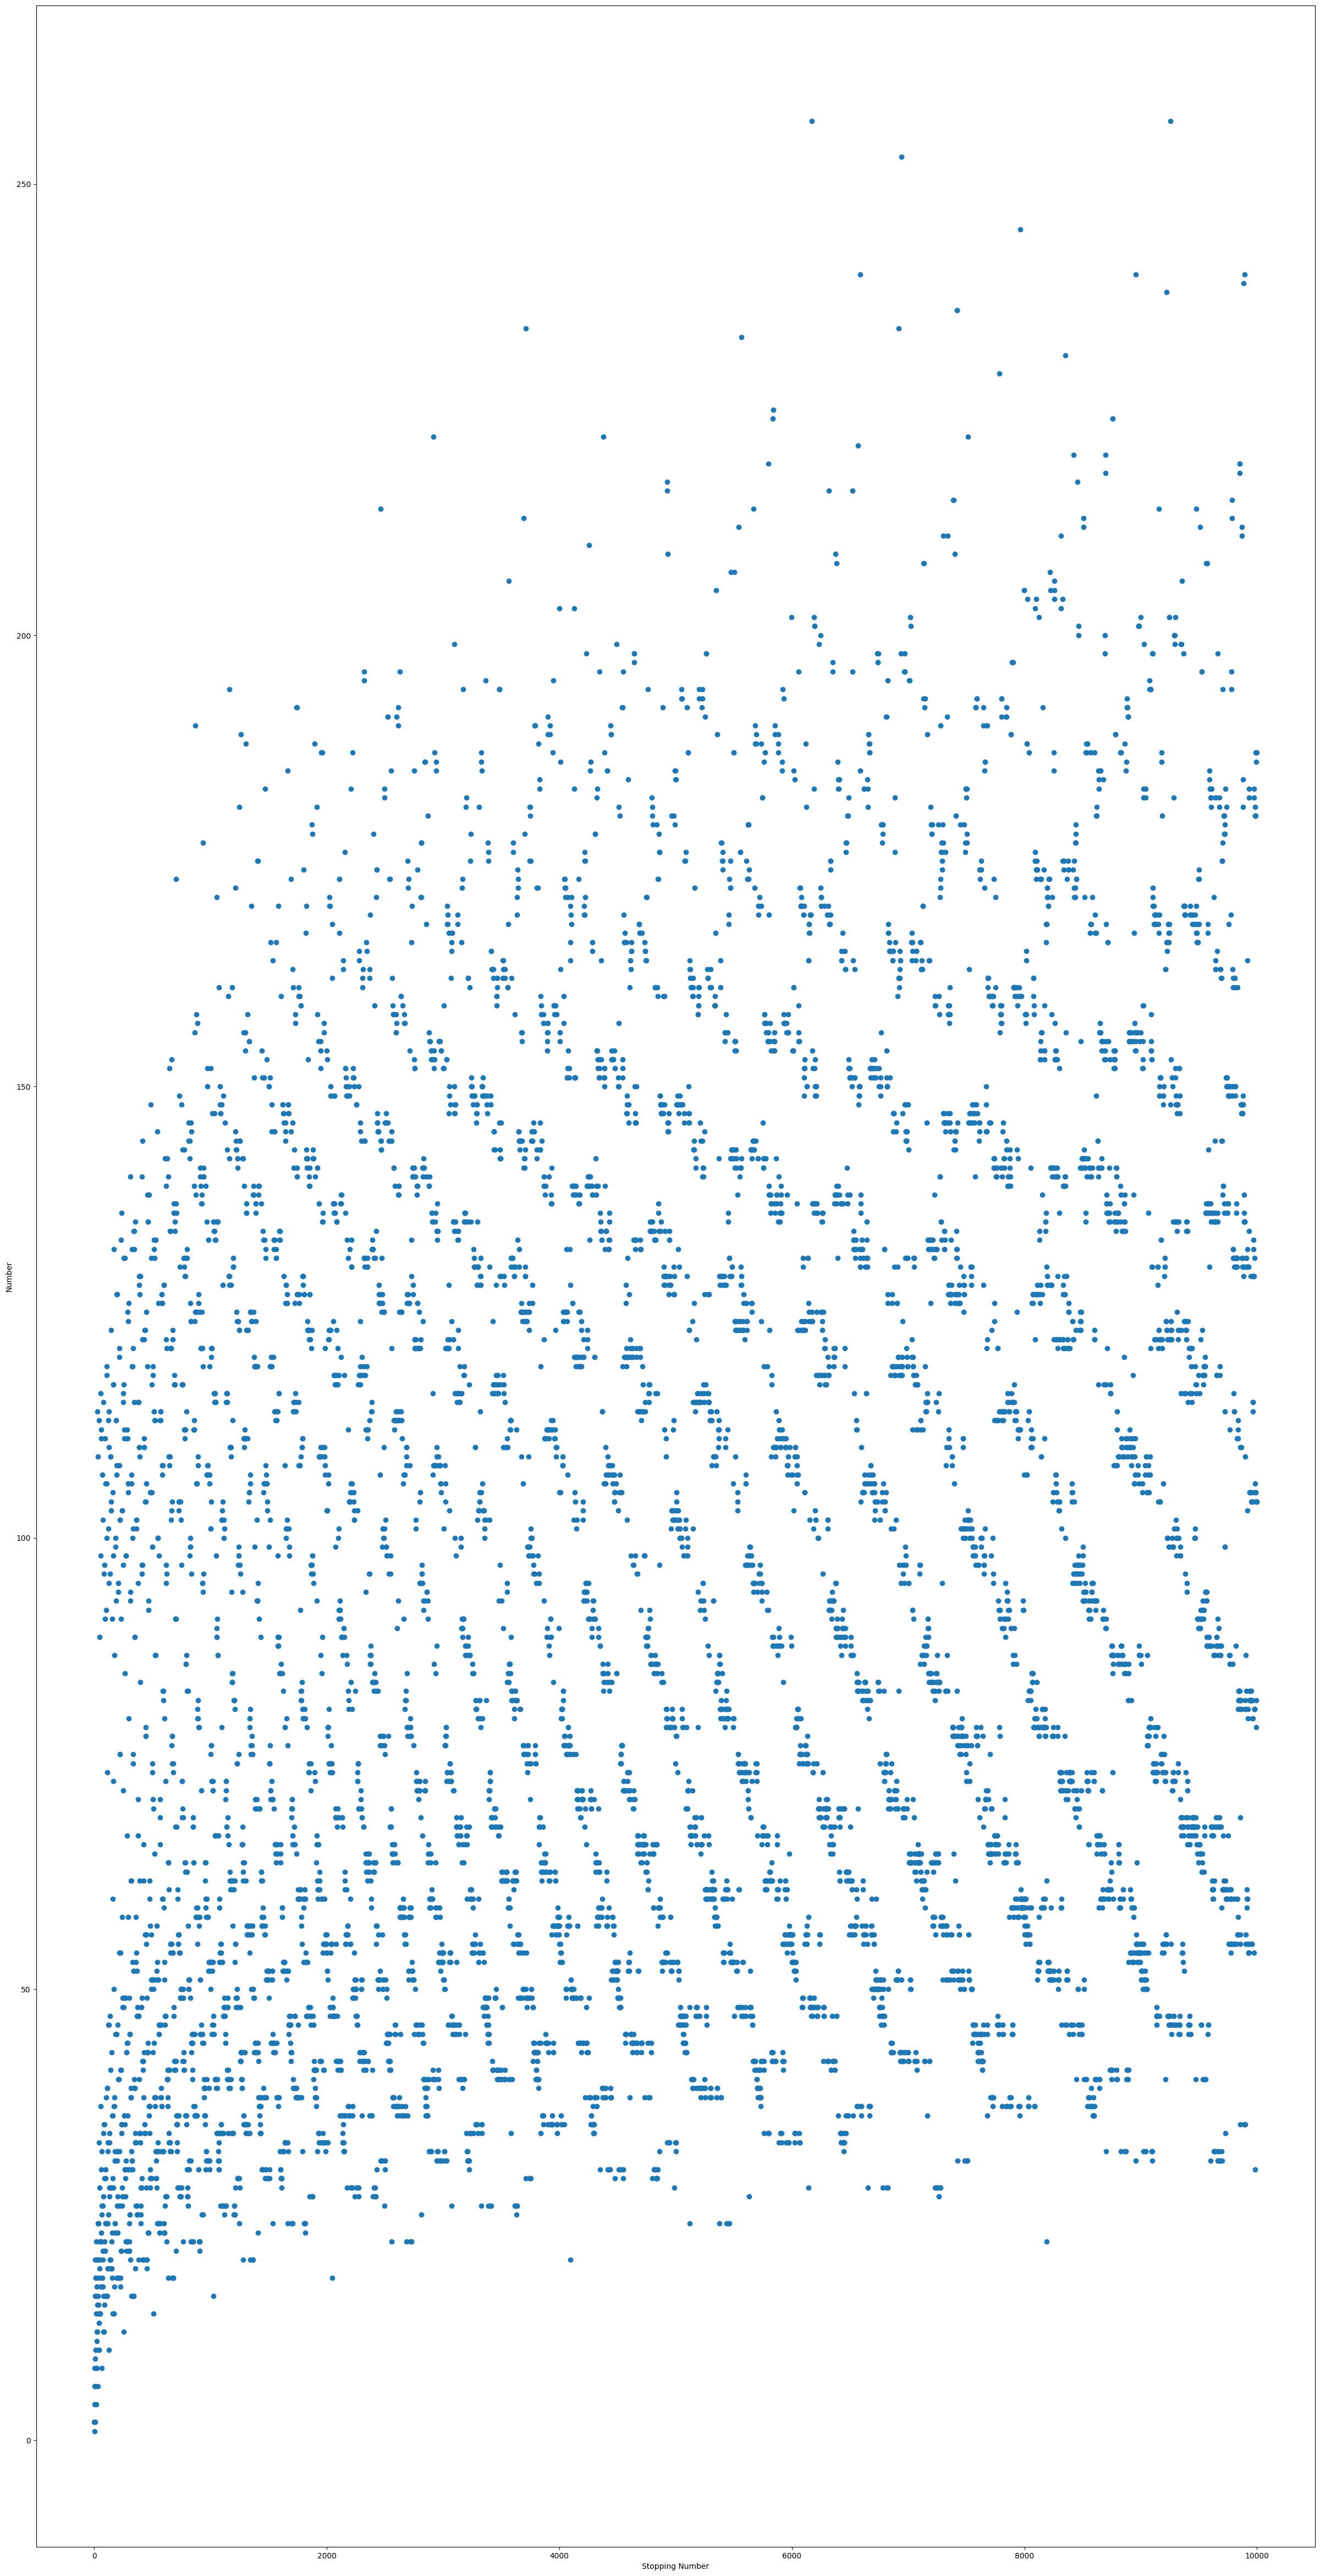
\includegraphics[height= 9 in]{images/10000 Collatz Stopping Times.png}
\end{centering}

As shown in the larger figure, the pattern does continue. Taking the log of the values in the hopes that it could clarify the stopping times gives the following graph, but the graph does not have a clearer pattern. 

\begin{wrapfigure}{R}{0.5 \textwidth}
\centering
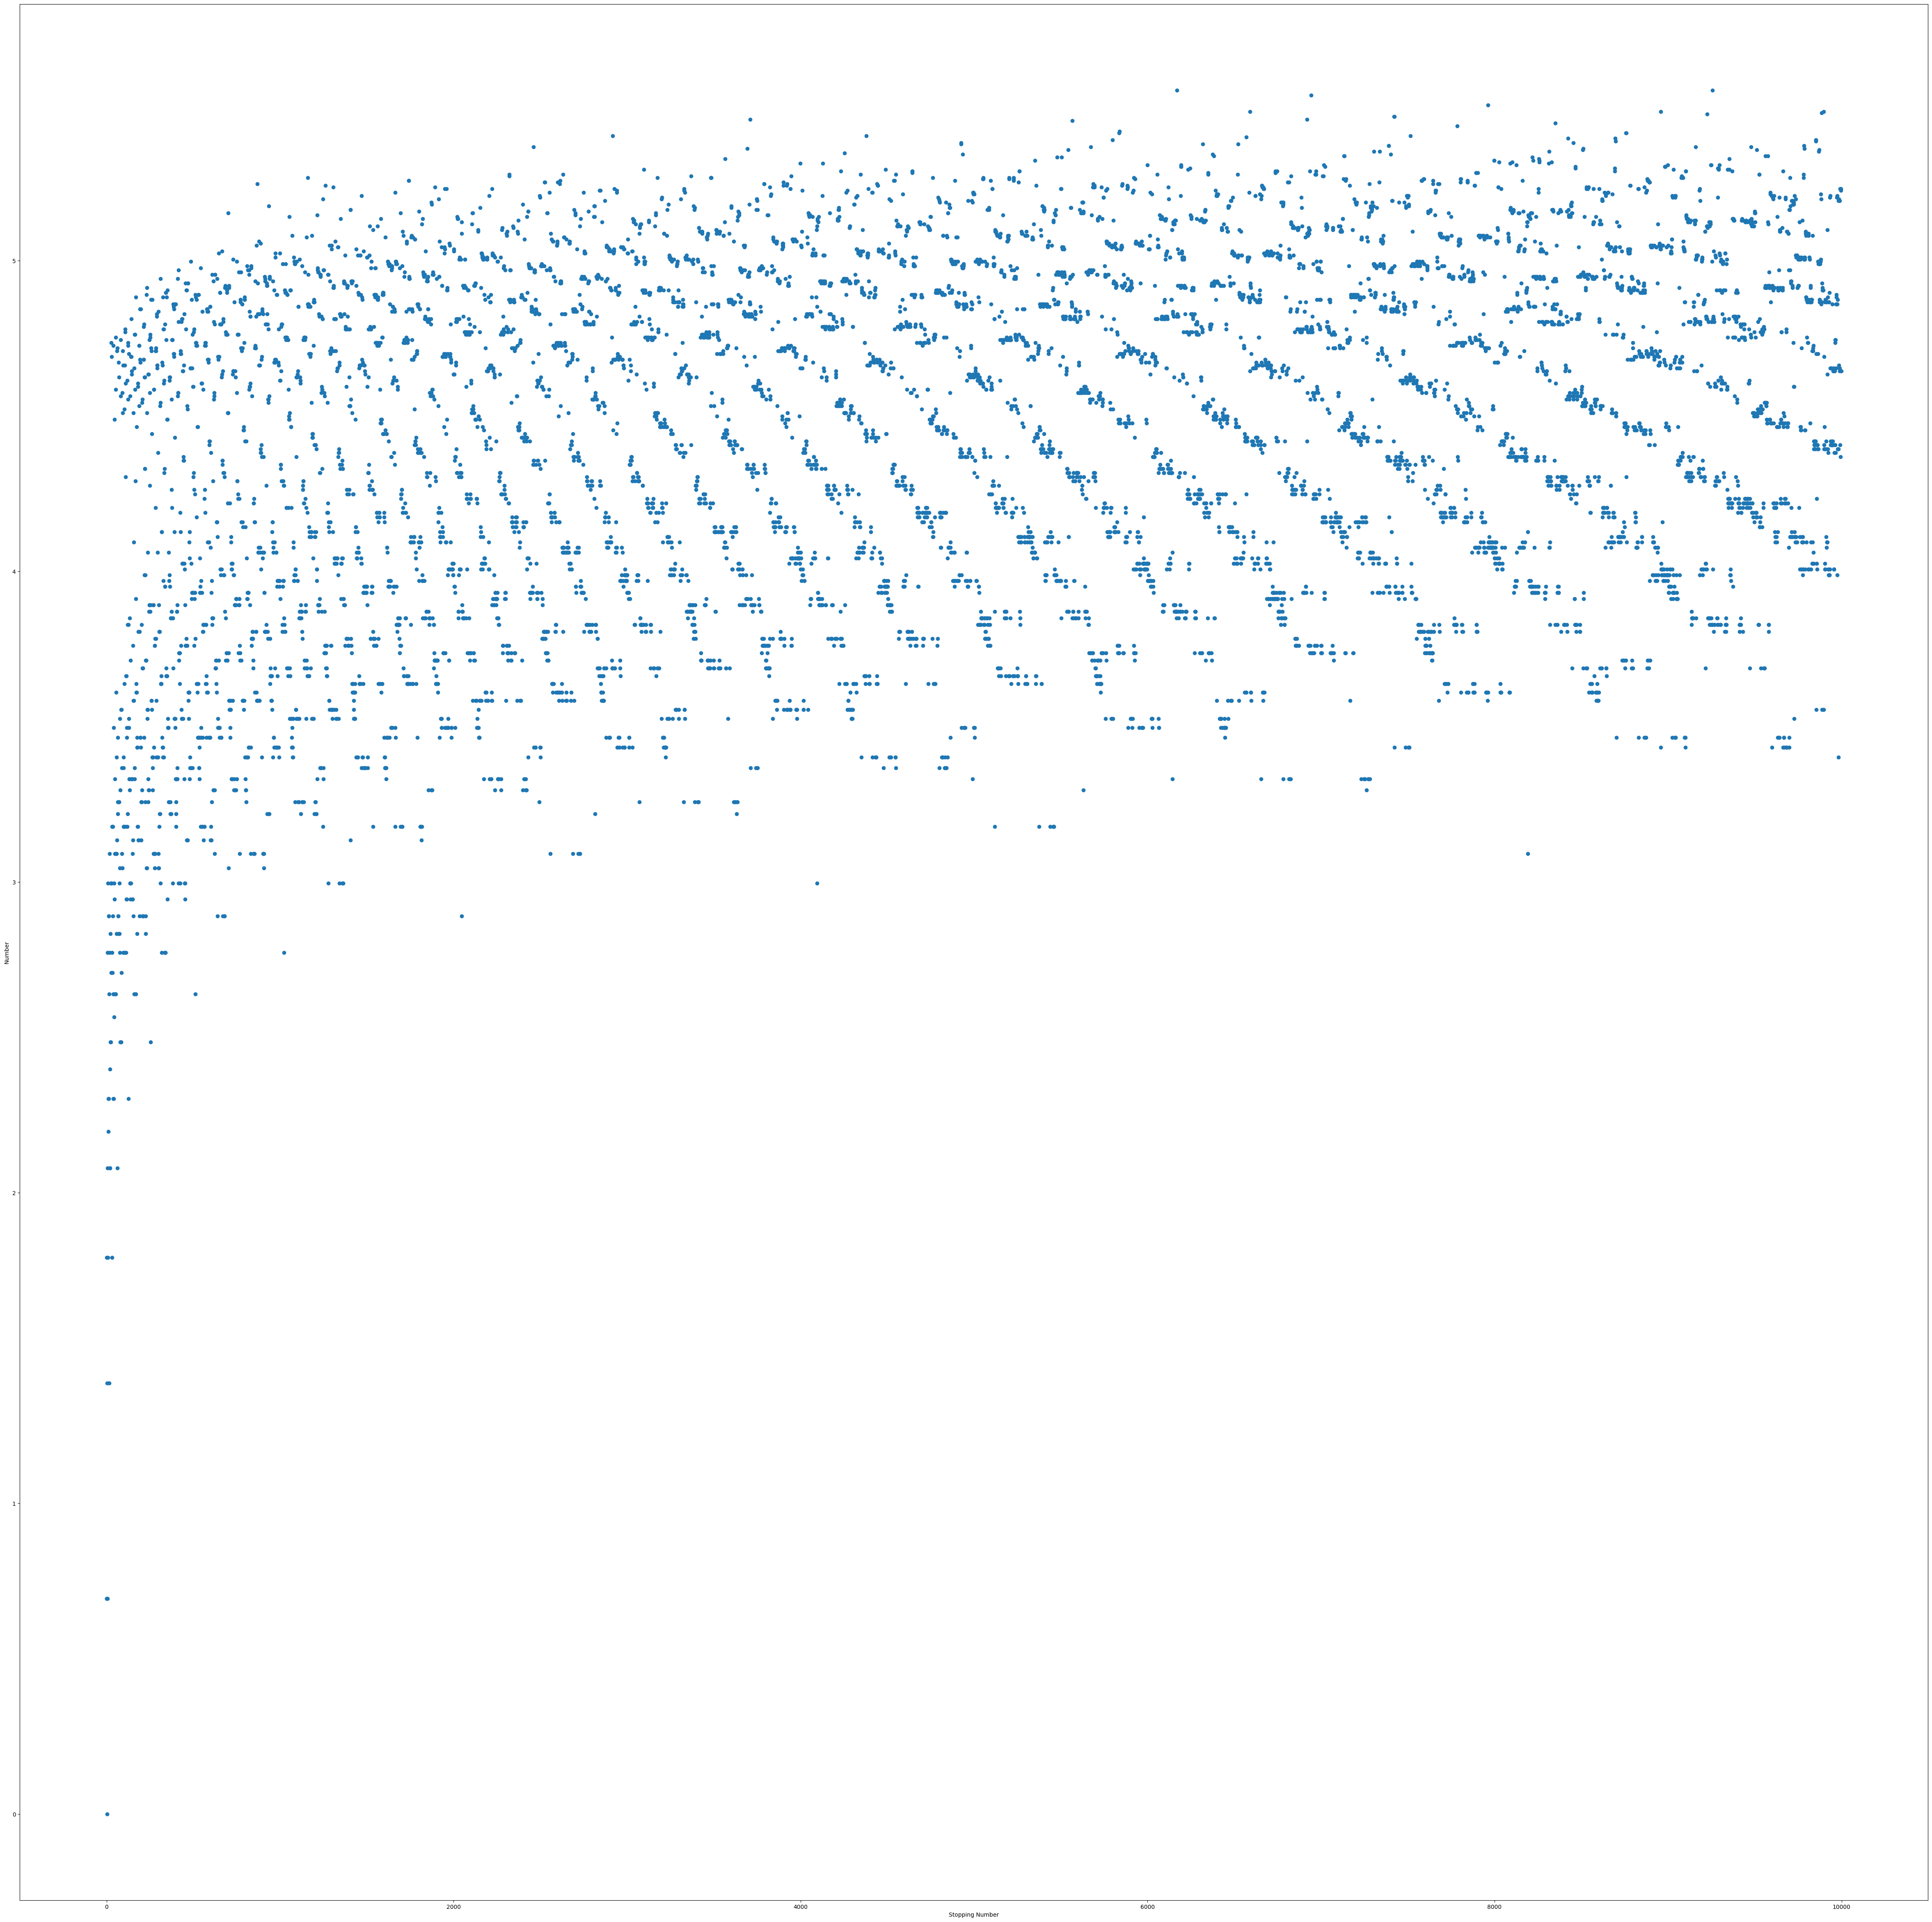
\includegraphics[width = 0.5 \textwidth]{images/10,000 log.png}
\caption{\label{fig:img3} Log of 10,000 stopping times}
\end{wrapfigure}

However, it is pretty cool to look at! 

The stopping times have been calculated for all $1 < n < 2^{68}$ as of 2022, and for all of these values, the Collatz conjecture reached 1. 

\end{document}
